\chapter{Geometria epipolarna}

W wizji stereoskopowej (ang. stereo vision) istnieją dwie metody odtwarzania
trójwymiarowości sceny. Pierwsza, klasyczna metoda, polega na odtworzeniu
struktury sceny z dwóch (lub więcej) ujęć o znanych parametrach soczewki i
wielkości matrycy (ang. camera resectioning) oraz położeniu ogniska w
przestrzeni naszego modelu. Da nam to możliwość oszacowania umiejscowienia
dowolnego punktu w przestrzeni na płaszczyźnie zdjęcia lub dowolnego punktu w
przestrzeni na podstawie dwóch linii od obydwóch ognisk przez obie projekcie
tego punktu. Metoda ta nie sprawdza się w sytuacji gdy parametry kamery się
zmieniają, np. w wyniku poruszenia lub zmiany otoczenia.  Druga metoda
polegająca na budowie linii epipolarnych, bliżej odpowiada działaniu systemów
występujących w naturze. W nieskalibrowanym (nieznanym) układzie, na podstawie
korelacji punktowych pomiędzy obrazami, wyznacza się macierz fundamentalną
(ang. fundamental matrix), dzięki której możemy odtworzyć ujętą scenę w
przestrzeni 3D. 

Obie te metody opierają się na tzw. triangulacji, procesie wyznaczającym punkt
w przestrzeni trójwymiarowej, na podstawie dwóch lub więcej dwuwymiarowych
projekcji tego punktu na płaszczyźnie. Mając dany obraz $I$, punkt
$M=($$^{W}X,$$^{W}Y,$$^{W}Z,$$1)^T$ (w układzie współrzędnych
$W$), musi leżeć na linii prostej, przechodzącej przez ognisko $O_C$ i obraz
danego punktu $m=(^{I}X,^{I}Y,1)^T$ na płaszczyźnie $I$. Szukany punkt $M$
znajduje się na przecięciu dwóch takich linii, otrzymanych z dwóch projekcji. 

\begin{figure}[h!] \centering
  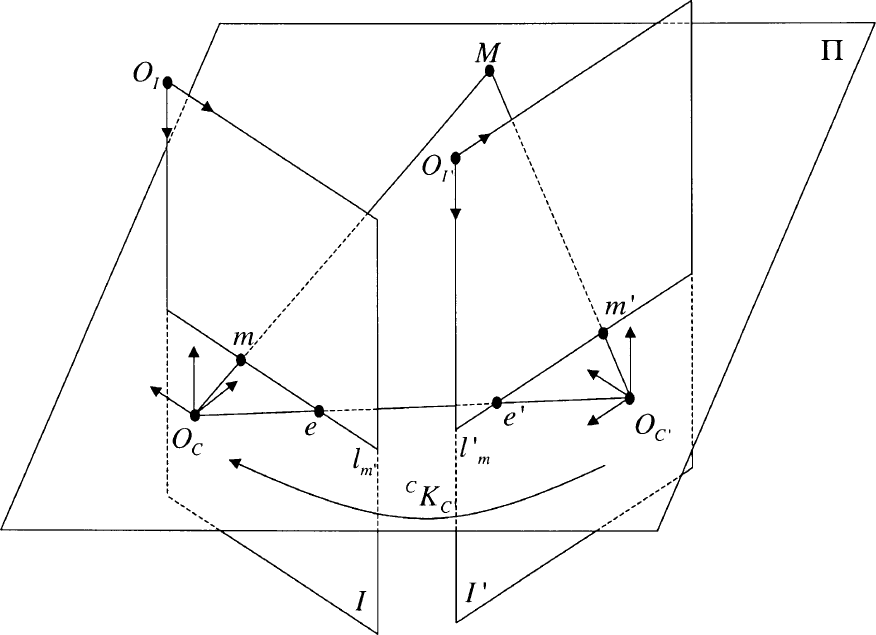
\includegraphics[width=1\textwidth]{images/epipolar_geometry.png}
  \caption{Przykładowa Geometria epipolarna. Schemat przedstawia dwie otworkowe
  kamery z ogniskami w punktach $O_C$ i $O_{C^\prime}$ widzące punkt $M$.
  Projekcje tego punktu na płaszczyznach $I$ i $I^\prime$ są oznaczone $m$ i
  $m^\prime$, epipole $e$ i $e^\prime$, a linie epopolarne $l_{m}$ i
  $l_m^\prime$. Macierz $^C K_C$ przekształca punkt $O_{C^\prime}$ w $O_C$ (o kąt i przesunięcie). Źródło: \cite{fm_overview} } \end{figure}

\section{Wyznaczanie macierzy fundamentalnej}

Macierz fundamentalna $F$ jest macierzą $3 \times 3$, która określa relacje
pomiędzy dowolnymi punktami $m$ i $m^\prime$ w wizji stereoskopowej, zgodnie ze
wzorem: 

\begin{equation}
  m^TFm^\prime = 0\,.
\end{equation}

H.C. Longuet-Higgins w publikacji "A Computer Algorithm for Reconstructing a
Scene From Two Projections" \cite{eight_point} opublikował tzw.  Eight-Point
Algorithm do wyznaczania macierzy fundamentalnej, na podstawie minimum ośmiu
par punktów $m_i=(u,v,1)$ i $m_i^\prime=(u^\prime,v^\prime,1)$.  Każda para,
tworzy jedno równanie liniowe, zawierające 9 niewiadomych, będących elementami
szukanej macierzy fundamentalnej $F$: 

\begin{equation} uu^\prime F_{11} + uv^\prime F_{21} + uF_{31} + vu^\prime
  F_{12} + vv^\prime F_{22} + vF_{32} + u^\prime F_{13} + v^\prime F_{23} +
  F_{33} = 0\,.  \end{equation}

Układ takich równań ma prostą postać w zapisie macierzowym:

\begin{equation} Af=0\,, \end{equation}

gdzie $f$ jest wektorem zwierającym 9 elementów macierzy $F$. Ponieważ $f$ jest
zdefiniowana z dokładnością dowolnego mnożnika skali, należy nałożyć dodatkowy
warunek, że norma $\|f\|$ jest równa 1. Z tego wynika, że do rozwiązania tego
układu równań wystarczy osiem par punktów.

Zaimplementowany przeze mnie algorytm rozwiązywania układów równań to
uproszczona metoda Jacobi-ego dla macierzy symetrycznych (gdyż macierz $A^TA$
zawsze jest symetryczna).

Ostatecznym rozwiązaniem jest wektor własny, odpowiadający najmniejszej
wartości własnej.  Wartości tego dziewięcioelementowego wektora tworzą macierz
fundamentalną o rozmiarze $3 \times 3$.

\section{Budowa linii epipolarnych}

Algorytm Random Sample Consensus (RANSAC) \cite{ransac} jest estymatorem,
którego celem jest dopasowanie odpowiedniego modelu do niepewnych
(doświadczalnych) danych wejściowych, obarczonych pewnym szumem lub błędem.
Jednym z zastosowań tego algorytmu jest budowa geometrii epopolarnej.
Publikacja "Enhancing RANSAC by generalized model optimization" \cite{loransac}
pokazuje, że jest możliwe odnajdywanie linii epipolarnych na podstawie jedynie
trzech par korespondujących regionów, ale tylko w połączeniu z takimi metodami
parującymi, które dopasowują całe kształty, z dokładnością do ich obrotu.
Dzięki temu będziemy mogli uzyskać trzy pary punktowych korespondencji pomiędzy
obrazami, dla każdej pary regionów.  Szacunkowy model geometrii epipolarnej
uzyskujemy losując trzy pary regionów korespondujących, z których otrzymamy
dziewięć par punktów niezbędnych do obliczenia macierzy fundamentalnej $F$.
Kolejnym krokiem jest przekształcenie wszystkich sparowanych punktów z obrazów
$I$ i $I^\prime$ macierzą $F$.  Algorytm LO-RANSAC \cite{loransac} (ulepszony
RANSAC) powtarzamy dla obu obrazów (na wejściu podając otrzymany zbiór
transformowanych punktów, oznaczany jako $\mathcal{U}$), który przebiega
następująco: \begin{enumerate} \item Losuj $m$ ze wszystkich $N$ punktów w
    zbiorze $\mathcal{U}$ (gdzie $m$ jest minimalną próbą niezbędną do
    określenia szukanego modelu; dla linii, $m$ jest równe 2). \item Zbuduj
    model na podstawie wylosowanych danych. Linię definiuje równanie: $y - y_1
    = (( y_2 - y_1 ) / ( x_2 - x_1 )) (x - x_1)$.  \item Sprawdź jak dużo
    punktów nie odbiega od modelu o więcej niż progowy parametr $\Theta$.
    Punkty leżące w linii (ang. inliners) zaliczamy do zbioru $\mathcal{I}$, a
    ich liczba to $I = |\mathcal{I}|$.  \item Jeżeli jest to najlepszy do tej
    pory szacunek ($I_k > I_j$ dla każdego $j < k$), zapamiętaj go. W
    przeciwnym razie przejdź do punktu 6. \item Wylosuj stałą liczbę punktów ze
    zbioru $I_k$ i przeprowadź optymalizację stosując algorytm IRLS
    (iteratively reweighted least squares). \item Jeżeli prawdopodobieństwo
    $\eta = (1-P)^k$, znalezienia lepszego modelu w $k$-tej próbie nie jest
    mniejsze od wartości progowej $\eta_0$ będącej parametrem, wróć do punktu
    1. W przeciwnym razie zwróć aktualny model. \end{enumerate}

Przyjmuje się, że para regionów jest spójna z wyznaczonym modelem, jeżeli
wszystkie jej trzy punkty są spójne. Prawdopodobieństwo $P$ wynosi: 

\begin{equation} P = \frac{{I \choose m}}{{N \choose m}} =
  \prod_{j=0}^{m-1}\frac{I - j}{N-j} \,.  \end{equation}

\section{Odtwarzanie przekształceń geometrycznych}

Sama macierz fundamentalna nie wystarczy do wyznaczenia w przestrzeni ani
położenia kamery, ani punktów korespondującym punktom na płaszczyźnie. Aby
jednoznacznie określić punkty w przestrzeni, konieczne są punkty zaczepne.
Według autorów "Stereo from Uncalibrated Cameras" \cite{stereo} może być to
dowolna para macierzy położenia kamer $P_1$, $P_2$ (ang. camera matrices),
która jest zdefiniowana przez:

\begin{equation}
  P_1 = \begin{pmatrix} 
    1 & 0 & 0 & 0 \\
    0 & 1 & 0 & 0 \\
    0 & 0 & 1 & 0
  \end{pmatrix}
;\quad P_2 = (U \begin{pmatrix} 
    r & 0 & 0 \\
    0 & s & 0 \\
    0 & 0 & \gamma
  \end{pmatrix} E V^T\; |\; U(0,0,\gamma)^T).
\end{equation}

W celu ich znalezienia, konieczne jest dokonanie rozkładu według wartości
osobliwych (ang. singular value decomposition) macierzy fundamentalnej $F$, w
formie $F = UDV^T$, gdzie $D$ jest macierzą diagonalną $diag(r,s,0)$. Ponieważ
w praktyce najmniejsza wartość własna $F$ nie będzie równa dokładnie 0, należy
tę wartość wymusić (po to, aby norma Euklidesowa była jak najbliższa $F$, a
jej rząd wynosił 2).  Macierze $P$ nie mają na celu dokładnego określenia
rzeczywistego położenia kamer w przestrzeni, a jedynie skojarzenie ich
położenia z trójwymiarową transformacją projekcji na płaszczyźnie.

Zgodnie z \cite{stereo} macierz $F$ można również rozpisać w następujący sposób:

\begin{equation}
  F = RS;\quad R = Udiag(r,s,\gamma)EV^T;\quad S = VZV^T ,
\end{equation}
gdzie 
\begin{equation}
  E = \begin{pmatrix} 
    0 &-1 & 0 \\
    1 & 0 & 0 \\
    0 & 0 & 1
  \end{pmatrix}
  ;\quad
  Z = \begin{pmatrix} 
    0 &-1 & 0 \\
    1 & 0 & 0 \\
    0 & 0 & 0
  \end{pmatrix},
\end{equation}
$R$ jest macierzą rotacji, a $\gamma$ niezerową wartością (zgodnie z
\cite{stereo} zawartą między $r$ i $s$).

\section{Odnajdywanie punktów w przestrzeni trójwymiarowej}

Współrzędne punktu ${\bf x_i} = (x_i, y_i, z_i) $ w przestrzeni, znajdują się
na przecięciu dwóch półprostych wyprowadzonych z ognisk obiektywu i
przechodzących przez dwie dwuwymiarowe projekcje w punktach $u_i = (u_i, v_i, 1)^T$ i
$u_i\prime = (u_i\prime, v_i\prime, 1)^T$. Przybliżone położenie tego punktu
można obliczyć w następujący sposób: 

\begin{equation} (w_i u_i, w_i v_i, w_i)^T = P_1(x_i, y_i, z_i, 1)^T
\end{equation} \begin{equation} (w_i\prime u_i\prime, w_i\prime v_i\prime,
  w_i\prime)^T = P_2(x_i, y_i, z_i, 1)^T \end{equation} Jest to układ sześciu
  równań z pięcioma niewiadomymi: $x_i, y_i, z_i, w_i$ i $w_i\prime$. Da on
  rozwiązanie z dokładnością do przekształceń rzutu.  Dokładne rozwiązanie
  (absolutne położenie) wymaga co najmniej ośmiu punktów zaczepnych w
  przestrzeni (ang. ground control points).

\section{Podsumowanie}

Uzyskana przez nas rekonstrukcja opiera się na projekcji i nie jest tzw.
rekonstrukcją euklidesową. To podejście pozwala na pomiar tzw. niezmienników
projekcji (ang. projective invariants) takich jak dwustosunek (ang.
cross-ratio) i przecięcia linii. Aby móc dokonać pomiarów kątów i odległości,
konieczna będzie kalibracja kamer. Problem ten został pominięty w tej pracy.
